\chapter{从传统虚拟化到虚拟容器}
\label{cha:virtualization-and-container}

虚拟化技术从 2008 开始越来越热,到了今天,已经成为了企业 IT 技术中必不可少的了。
本章节首先介绍虚拟化技术的演变以及在发展过程中产生的几种类型,然后介绍几种用户
层 (user-land) 的虚拟化管理工具,然后介绍本次实验采用的宿主系统 CentOS 7 的
一些特性,最后罗列 OpenStack 支持的几种虚拟化方案。

在下文中,如果没有特殊说明,用虚拟机管理程序指代 hypervisor ,用宿主机
指代 host ,也就是承载虚拟机管理程序的物理机器和上面运行的操作系统,用
客户机或者客户虚拟机指代 guest ,也就是运行在宿主机上由虚拟机管理程序
模拟出的环境上的宾客操作系统及相关软件。

\section{虚拟化技术的演变}

和其它大多数技术一样,虚拟化技术也不是一蹴而就的,它经历了以下几种形态的演变和发展
~\cite{deep-into-kvm}:

\subsection{软件模拟}
\label{emulators}

严格来说,模拟器 (emulator) 不是一种虚拟化方式,但是它也可以实现在宿主机上
运行不同的客户机操作系统。它的出现早于虚拟化技术,而且实现的方式形形色色,例如
早期的 Macintosh 电脑可以安装兼容 DOS 系统的扩展卡,从而运行为 PC 编写的
程序。现在常见的形式是软件模拟,例如 QEMU \footnote{QEMU 可以和 KVM 配合,
工作在 virtualizer 模式,在这里只讨论 emulator 模式}。

\begin{figure}[h]
    \centering
    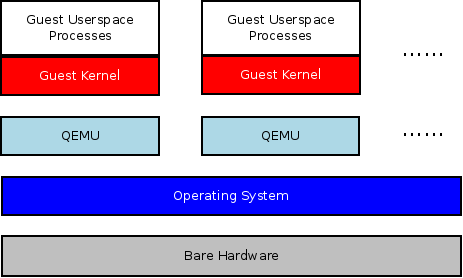
\includegraphics[width=0.7\textwidth]{qemu-arch}
    \caption{QEMU 的基本结构}
\end{figure}

和 Bochs 不同,QEMU 不仅能模拟 X86 架构的处理器,还能支持 ARM / MIPS / PowerPC
 / Sparc / Xtensa 等多种架构的处理器~\cite{qemu-internals}。
而且 QEMU 和 Valgrind 一样使用的是动态翻译。所谓静态翻译,就是不需要执行程序本身,
一次读入整个二进制文件,完成翻译;所谓动态翻译,就是在执行过程中只看一小段程序,
比如一个基本块 (basic block) ,然后翻译并缓存 (caching)翻译好的目标代码。
这样的好处是二进制程序只在需要的时候被翻译,比如一个循环,执行一次之后
又跳转回到和一开始相同的代码,那么只需要指向缓存中已经翻译好的代码就可以了,
而不用重新翻译一遍。

当然 Valgrind 本质上是一个检查内存错误的 memcheck 工具,这是它和 QEMU 根本上的不同。
如果模拟器工作在纯软件模拟,执行效率是不高的,但是好处是理论上可以模拟任何硬件,
以至于不存在的硬件。

\subsection{虚拟化层翻译}

\subsubsection{软件全虚拟化}
\label{subsubsec:software-virt}

成立于 1998 年的 VMWare 最早提出了软件虚拟化的概念。和~\ref{emulators}小节提到的
模拟器不同,VMWare 的虚拟机管理程序不需要模拟物理上并不存在的硬件的指令集系统,既不像
静态翻译一样需要一个接一个地把程序的 CPU 指令翻译成宿主机上的指令,也不像动态翻译一样
需要在基本块第一次运行的时候翻译整段代码。但是 VMWare 需要虚拟各种硬件适配器,例如
网络适配器、图形适配器或者磁盘。

VMWare 的出现远早于 Intel 或是 AMD 的硬件虚拟化扩展 (Intel VT 或是 AMD-V),
那么最初的 VMWare 是怎么靠纯软件的方法实现虚拟机管理程序的呢?
本科操作系统课讲过,X86 处理器的指令划分为 4 个特权级,
也就是 Ring 0 、Ring 1 、Ring 2 和 Ring 3 。操作系统和一些设备驱动的特权级最高,
一般使用 Ring 0 ,用户态 (user-mode) 程序特权级比较低,一般使用 Ring 3 。
Ring 1 和 Ring 2 很少使用。当然,这取决于操作系统内核的设计,比如
OS/2 使用三个 Ring —— 内核和驱动使用 Ring 0,可以访问 I/O 的特权程序使用
Ring 2 ,普通用户态程序使用 Ring 3;OpenVMS 使用全部四个 Ring 。
而软件实现虚拟化,就是要对客户机的越级指令进行隔离,这样一来,
虚拟机管理程序上运行的客户机虽然运行的是和宿主机相同的指令,但是客户机的越级指令
也不能直接操作硬件。比如用户重启虚拟机不会导致宿主机也重启。

VMWare 虚拟机管理程序对客户机代码的执行分为两种情况,一种是执行用户态 (user-mode)
或者虚拟 8086 模式 (virtual 8086 mode),那么代码将会直接执行;另一种是执行
内核级别或者实模式 (real-mode) 的代码,这时候就需要转换和改写原有的代码。
VMWare 的改写是动态的,转换以后的代码存储在一块特殊的地址区域,通过内存分段机制
保护起来。

当然,随着虚拟化技术的发展,现代的 Intel 和 AMD 处理器都支持硬件虚拟化扩展,
所以较新版本的 VMWare 软件也支持硬件虚拟化了,不再是上文介绍的纯粹软件的
实现方式。对于硬件虚拟化,会在~\ref{subsubsec:hardware-virt}小节进行
介绍。

\subsubsection{半虚拟化}
\label{subsubsec:paravirtualization}

上文提到的纯软件的全虚拟化,比如 VMWare ESX ,实际上是存在效率问题的,
这是因为虚拟机管理程序必须对客户虚拟机的整个内核的代码中的非陷入 (non-trapping)
的特权指令进行修改,而且是动态修改。在 2003 年的 ACM SOSP 上,一种叫 Xen 的
新型虚拟化技术被剑桥大学的计算机科学家提出出来~\cite{barham2003xen}。

Xen 解决越级指令的办法,是将客户虚拟机的内核放在 Ring 1 执行,这是可行的,因为
~\ref{subsubsec:software-virt}提到,现代的大多数 X86 平台的操作系统都
只使用 Ring 0 执行内核代码和 Ring 3 执行用户态代码。符合这个条件的操作系统,
比如 GNU/Linux 、Windows XP 和 BSD \footnote{在 2003 年的 Xen 1.0 版本中,
事实上只有 GNU/Linux 内核是基本工作正常的,Windows 支持做了一部分,
NetBSD 则几乎不能工作},理论上都可以被移植 (port) 到 Xen 上。

\begin{figure}[h]
    \centering
    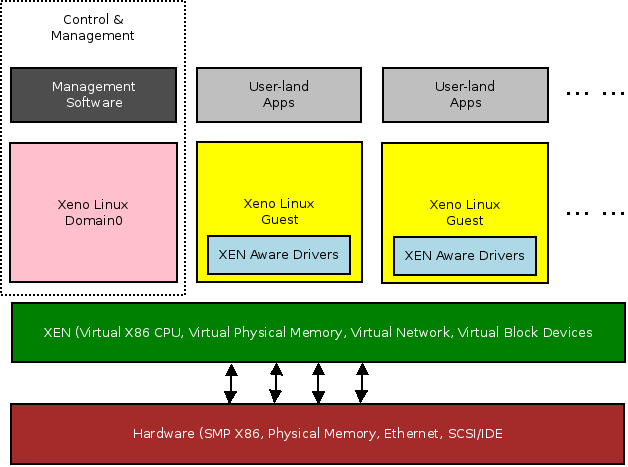
\includegraphics[width=0.8\textwidth]{xen-arch}
    \caption{Xen 的架构}
\end{figure}

那么 Xen 是如何解决性能问题的呢?通常来讲,两种异常 (exception)的频繁发生会显著
影响系统性能,也就是一般用软件异常 (softwareexception) 实现的系统调用,
以及缺页异常。Xen 上运行的客户虚拟机的系统调用的效率通过允许客户机注册一个
可以由进程直接访问而不用通过 Ring 0 的异常处理函数 (exception handler) 来
提高。但是缺页异常就不能这样做,因为要访问 CR2 寄存器。所以缺页异常的处理必须通过
Xen 本身,使得 CR2 被正确设置,并且能从 Ring 1 正确被客户虚拟机的内核访问。

这样一来就带来了一个问题,客户虚拟机的内核必须要进行修改,来让自己“意识”到自己是在
Xen 虚拟机管理程序而不是裸硬件上运行的。Xen 的作者管这样的虚拟化技术叫“半虚拟化”,
区别于不需要修改客户虚拟机内核的全虚拟化技术。半虚拟化的好处是客户机负载运行效率
要比早期的软件全虚拟化更高,坏处是需要使用一个修改过的内核,而且不是所有的内核都可以
使用和 GNU/Linux 同样的方式,有的操作系统需要的精力更大一些。

Xen 使用了 X86 架构的特性,但是它还是软件实现的,并没有改变处理器的架构。

\subsubsection{硬件支持的全虚拟化}
\label{subsubsec:hardware-virt}

\begin{figure}[h]
    \centering
    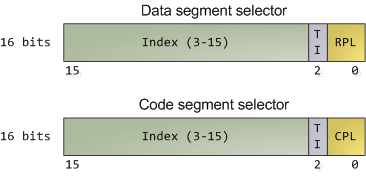
\includegraphics[width=0.7\textwidth]{segment-selectors.png}
    \caption{X86 的段寄存器}
\end{figure}

\begin{table}[h]
    \centering
    \caption{X86 中的状态标志寄存器 FLAGS}
    \begin{tabular}{||c c c||}
        \hline
        Bit & Abbr & Description \\
        \hline
        \hline
        0 & CF & Carry flag \\
        1 &  & Reserved \\
        2 & PF & Parity flag \\
        3 &  & Reserved \\
        4 & AF & Adjust flag \\
        5 &  & Reserved \\
        6 & ZF & Zero flag \\
        7 & SF & Sign flag \\
        8 & TF & Trap flag \\
        9 & IF & Interrupt enable flag \\
        10 & DF & Direction flag \\
        11 & OF & Overflow flag \\
        12-13 & IOPL & I/O privilege level (286+ only, all 1 otherwise) \\
        14 & NT & Nested task flag (286+ only, 1 otherwise) \\
        15 &  & Reserved \\
        \hline
    \end{tabular}
    \label{table:flags-x86}
\end{table}

传统的 X86 架构对于虚拟化主要有两个阻碍~\cite{adams2006comparison}:

\begin{itemize}
    \item 客户机操作系统可以观察到自己处于非特权状态。X86 的代码段寄存器 CS 的最低两位存储的
    就是当前的特权级 (CPL, current privilege level);
    \item 当特权指令运行在非特权模式,也就是用户态 (user-level) 的时候,缺乏相应的陷入。
    我们知道,X86 里的 FLAGS 寄存器一共有 16 位,参见表~\ref{table:flags-x86}。
    如果运行特权指令 popf 的话,那么控制ALU 的 ZF 位和控制系统的 IF 位
    \footnote{中断使能}都会被修改。客户虚拟机的内核必须触发陷入虚拟机
    管理程序才能修改虚拟的 IF 寄存器位,但是事实上如果直接在用户态运行 popf ,那
    陷入就不会发生,虚拟机管理程序无从知晓 IF 应该被修改这个事实。
\end{itemize}

Intel 的 VT 和 AMD 的 AMD-V 技术对 X86 的结构做出了一些扩展,使得其更好地支持虚拟化技术,
这就是“硬件支持的全虚拟化”这个术语的含义。

首先在内存中引入了一个虚拟机控制块 VMCB ,主要存贮客户虚拟机的状态信息和一些控制位。然后 X86
处理器又增加了一个客户模式 (guest mode) 负责运行客户虚拟机的代码,尤其是特权代码。从宿主模式
转变到客户模式需要使用一个全新的指令,vmrun 。

那么如何判断自己的硬件是否支持硬件虚拟化技术呢?以本文作者目前使用基于 Haswell 架构的
的戴尔 Chromebook 为例,/proc/cpuinfo 的输出中含有 vmx 标记位,就证明处理器支持
 Intel 的硬件虚拟化技术。截至 2015 年,大部分 Intel 的处理器都支持这个功能。

 \begin{figure}[h]
     \centering
     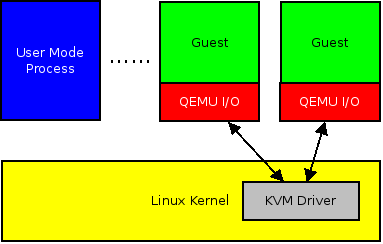
\includegraphics[width=0.7\textwidth]{qemu-kvm-arch.png}
     \caption{QEMU-KVM 的架构示意}
 \end{figure}

一些新兴的虚拟机管理程序必须要求宿主机支持硬件虚拟化技术,比如开源内核的模块 KVM ,它和 QEMU
结合紧密,由 QEMU 提供模拟的硬件设备,所以一般称为 QEMU-KVM 。KVM 技术和 Linux 内核结合
较好,又天生支持硬件虚拟化,还有商业公司 Red Hat 提供技术支持,可以说是虚拟化界的新秀。

\subsection{容器虚拟化}

容器虚拟化的技术实现和上文提到的各种虚拟化技术有很大的不同。而且现在业界对于什么样的虚拟化
技术可以归类为“容器”也没有统一的说法,一个笼统的概念是容器是一个相对独立的运行环境。
容器内部的进程可以使用宿主机的资源,但是又不能把宿主机的资源全部消耗掉,而且其运行环境必须
和宿主机有一定的隔离,最小化对外界的影响,比如说虽然有容器内部的 root 权限,但是仍然
有很多会影响宿主机的操作不能执行。

类似的技术在很多操作系统上都有实现,比如 FreeBSD 上的 jail 或是 Solaris 上的 Zone ,
但是容器技术普及推广开来,还是因为 Linux 虚拟容器。这里需要说明,我们通常说的 LXC 包含
两层意思,一层是指 Linux 内核中对虚拟容器技术的实现,主要包括下文所说的命名空间 (namespace)
和控制组 (cgroup) ,另外一层是指 LXC 的用户态管理工具,这个是次要的,但是是和用户经常打交道
的部分。

\subsubsection{命名空间}

命名空间 (namespace) 技术主要是用于访问隔离,主要包括\footnote{从 Linux kernel
 3.8 开始}六种——Mount Namespace 、PID Namespace、Net Namespace、IPC Namespace、
UTS Namespace 还有 User Namespace ~\cite{docker-in-practice}。

\begin{itemize}
    \item \textbf{Mount Namespace} 用来隔离文件系统的挂载点,每个进程看到的文件系统会
    被记录在 /proc/\$\$/mounts 里。这样的话,对于一个 Linux 虚拟容器,在容器内部挂载
    或者卸载文件系统就不会影响到容器外的部分。之后我们会看到这个特性如何运用在 NOVA 对
    procfs 的处理中;
    \item \textbf{PID Namespace} 用来隔离不同命名空间之中的进程号 (PID) ,这样,
    在不同的命名空间就可以使用同一个进程号了。举最简单的例子,init 进程的 PID 是 1 ,
    那每个容器里开机肯定都会跑 init 进程,如何区分 PID 都是 1 的进程属于哪个容器,
    这就是 PID Namespace 的工作了;
    \item \textbf{Net Namespace} 用来隔离不同的命名空间之间的网络设备、路由表、端口号
    等网络相关的信息;
    \item \textbf{IPC Namespace} 主要用于管理不同的命名空间的 SysV IPC 标示符还有
    POSIX 消息队列;
    \item \textbf{UTS Namespace} 用来隔离命名空间的主机名和域名。之所以叫 UTS
    是因为存储这些信息的结构体叫做 utsname 。
    \item \textbf{User Namespace} 用来隔离命名空间之间的用户和用户组。举例来说,
    多个容器可能都有 root 用户,这是非常正常的。但凡是 root 它的 UID 和 GID 都是 0 ,
    那么如何区分“这个” root 账户是属于那个容器的这个任务就由 User namespace 负责。
    这样,root 用户的权限只能限制在容器内部,而不能对宿主机进行特权操作。
\end{itemize}

那么命名空间有什么作用呢?比如在容器内部执行 hostnamectl set-hostname 操作
\footnote{这个命令是 systemd 风格的,其它发行版可能有不同的命令,不过它们使用的
系统调用都是相同的}设置主机名,那么宿主机的主机名还是保持原先的不变。这就是 UTS Namespace
在起作用。

\subsubsection{控制组}

控制组 (cgroup) 技术就是控制一组进程对系统资源使用的一种技术,它是 Linux 内核的组成部分,
已经被 Android 和目前绝大多数 Linux 发行版默认开启。Cgroup 可以管理的系统资源包括 CPU 、
内存、I/O 等,而不同种类的资源的管理是由不同的模块实现的,主要包括以下几个模块:

\begin{itemize}
    \item \textbf{cpu:} 这个子系统主要用于限制一个进程组对 CPU 资源的占用,主要包括
    三个方面:
    \begin{itemize}
        \item CPU 比重分配。比如有两个 cgroup ,cpu.shares 相同,那么如果两者争抢
        CPU 资源,它们得到的 CPU 占用率上限配额是相同的;如果其中一个 cpu.shares 是
        另一个的两倍,那么在抢占的时候前者最多可以得到后者两倍的 CPU 占用;
        \item CPU 带宽限制。cpu.cfs\_period\_us 和 cpu.cfs\_quota\_us 两个参数的意思是
        一个 cgroup 的进程在 cfs\_period 的时间内最多只能运行 cfs\_quota 这么多“配额”
        的时间,然后就会被强制睡眠直到下一个 cfs\_period 长度的时间片的到来。两者的单位
        都是微秒;
        \item 实时进程的带宽限制。使用 cpu.rt\_period\_us 和 cpu.rt\_runtime\_us 两个
        参数,方法和上面相似。
    \end{itemize}
    \item \textbf{cpuset:} 进程组使用的 CPU 和内存节点。
    \item \textbf{memory:} 这个子系统主要管理进程组能使用的内存资源,有如下几个重要
    参数:
    \begin{itemize}
        \item memory.limit\_in\_bytes: 设置内存使用上限,单位是 Bytes ;
        \item memory.memsw.limit\_in\_bytes: 和上面的类似,但是加上交换 (swap) 空间;
        \item memory.oom\_control: 设置为 0 来防止因为内存不足杀死进程。内存不足
        无法运行的进程将阻塞直到系统释放出足够的内存供使用。另外,将通知用户态。
    \end{itemize}
    \item 另外还有 devices 、net\_cls 、huge\_tlb 等多个 cgroup 子系统。它们的功能
    都是控制资源被进程组的使用,作用都是类似的,所以在这里不再赘述。
\end{itemize}

\section{OpenStack 支持的虚拟化类型}

在~\ref{subsubsec:iaas}小节提到过,OpenStack 是一个开放的虚拟化“基础设施即服务”的平台,
其中 OpenStack Nova 是负责虚拟机管理和计算的部分。那么,这个功能强大的基础设施平台究竟支持
什么样的虚拟机管理程序呢?

OpenStack Nova 对于虚拟机管理程序做了一个抽象层,这样,不同的虚拟机管理程序可以通过
compute-driver 的形式整合进 OpenStack Nova 中。因为不同的虚拟化技术诞生有先后,
OpenStack 对它们的支持程度和测试的详尽程度也不尽相同,分类来讲主要可以划分成以下三个
层次:

\begin{enumerate}
    \item \textbf{Group A:} 这一组的虚拟机管理程序经过了完整的单元测试 (unit test)
    和功能测试 (functional test) ,达到了基本上可用的程度。不过很遗憾目前只有一个:
    \begin{itemize}
        \item X86 平台的 QEMU-KVM
    \end{itemize}
    \item \textbf{Group B:} 这一组的虚拟机管理程序通过了完整的单元测试和部分的功能测试:
    \begin{itemize}
        \item Hyper-V
        \item VMWare
        \item XenServer
        \item Xen on libvirt
    \end{itemize}
    \item \textbf{Group C:} 很少的单元测试、几乎没有功能测试,
    可以认为是\textbf{不可用}:
    \begin{itemize}
        \item docker
        \item LXC on libvirt
    \end{itemize}
\end{enumerate}

那么,有没有一个用户友好的虚拟机管理软件栈能较好的支持新兴的 Linux 虚拟容器技术呢?
这就是下文要介绍的 Tsinghua NOVA 系统。
